%!Mode:: "TeX:UTF-8"
\documentclass[a4paper,12pts]{article}

\usepackage[polish]{babel}
\usepackage[utf8]{inputenc}
\usepackage{fontspec}
\setmainfont{Calibri}

\linespread{1.15}

\usepackage{caption}
\captionsetup{%
	font={footnotesize},
	labelfont={bf}
}

\usepackage{anysize}
\usepackage{geometry}

\usepackage{graphicx}

% Plik szablonowy do wykorzystania pózniej - nie zmieniaj go!

\begin{document}
	\thispagestyle{empty}
	\begin{flushleft}
		Wydział Elektrotechniki, Automatyki, Informatyki i Inżynierii Biomedycznej \\
		Informatyka, rok II \\
		Zespół numer 3 \\
		Piotr Kucharski \\
		Dominik Zabłotny \\
		\vspace*{\fill}
		%-----------NUMER CWICZENIA--------%
		{\large \textbf{Sprawozdanie z ćwiczenia nr 32} } \\
		%-----------TEMAT ĆWICZENIA--------%
		Mostek Wheatstone'a		
		\vfill	
		%-----------DATA-------------%
		25 października 2017r
	\end{flushleft}
	
	\newpage
	
%--------------------------------------------------------------------------------------------------------------
	
	\section{Wstęp}
	
	\subsection{Cele ćwiczenia}
	
	Celem wykonywanego ćwiczenia jest praktyczne zastosowanie prawa Kirchhoffa oraz sprawdzenie zależności określających opór zastępczy dla połączeń szeregowych i równoległych.
	
%--------------------------------------------------------------------------------------------------------------
	
	\subsection{Wprowadzienie teoretyczne}
	
	\subsubsection{Pierwsze Prawo Kirchhoffa}
	
	\textit{Twierdzenie o punkcie rozgałęzienia.} Algebraiczna suma natężeń prądów przepływających przez punkt rozgałęzienia (węzeł) jest równa zeru:
	
	\begin{equation}
		\sum_{i=1}^{n} I_{i} = 0
	\end{equation}
	
	Twierdzenie o punkcie rozgałęzienia wynika z zasady zachowana ładunku.
	
%--------------------------------------------------------------------------------------------------------------	
	
	\subsubsection{Drugie Prawo Kirchhoffa}
	
	\textit{Twierdzenie o obwodzie zamkniętym.} Algebraiczna suma sił elektromotorycznych i przyrostów napięć na dowolnym obwodzie zamkniętym jest równa zeru (spadek napięcia jest przyrostem ujemnym napięcia):
	
	\begin{equation}
		\sum_{i=1}^{n} \varepsilon_{i} + \sum_{i=1}^{m} I_{i} R_{i} = 0
	\end{equation}
	
	Twierdzenie o obwodzie zamkniętym wynika z zasady zachowania energii.
	
%--------------------------------------------------------------------------------------------------------------	

	\subsubsection{Opór elektryczny}
	
	Opór elektryczny $R$ (\textit{Rezystancja}) to wielkość charakteryzująca relacje między napięciem a natężeniem prądu elektrycznego w obwodach prądu stałego. Najczęściej mówi się, że opór elektryczny jest to zdolność materiału do przewodzenia prądu, który definiujemy wzorem:
	
	\begin{equation}
		R = \frac{U}{I} \textrm{ [$\Omega$]}
	\end{equation}

	gdzie:
	\begin{itemize}
		\item $R$ ~-- opór elektryczny [$\Omega$]
		\item $U$ ~-- napięcie prądu [V]
		\item $I$ ~-- natężenie prądu [A]
	\end{itemize}

%--------------------------------------------------------------------------------------------------------------
	
	\subsubsection{Opór właściwy}
	
	Opór właściwy $\rho$ (\textit{Rezystowność}) to wielkość charakteryzująca materiały pod względem przewodnictwa elektrycznego. Określana jako trudność na jaką jaką natrafiają przemieszczające się elektrony. Opór właściwy zależy od długości przewodu, jego przekroju poprzecznego oraz materiału z jakiego został wykonany. Rezystowność definiujemy wzorem:
	
	\begin{equation}
		\rho = \frac{R \cdot S}{l} \textrm{  [$\Omega \cdot$ \textrm{m}]}
	\end{equation}

	gdzie: 
	\begin{itemize}
		\item $\rho$ ~-- opór właściwy [$\Omega \cdot \textrm{m}$]
		\item $R$ ~-- opór elektryczny [$\frac{\textrm{kg} \cdot \frac{\textrm{m}^{2}}{\textrm{s}^{2}}}{\textrm{A} \cdot \textrm{s}}$]
		\item $S$ ~-- pole przekroju poprzecznego [\textrm{m}$^{2}$]
		\item $l$ ~-- długość elementu [m]
	\end{itemize}

%--------------------------------------------------------------------------------------------------------------

	\subsubsection{Zależność oporności elektrycznej metali od temperatury}
	
	Pomiędzy opornością elektryczną w metalach a temperaturą zachodzi relacja, którą tłumaczymy zmianą oporności metalu przy zmianie temperatury o 1 K. Zależność rezystancji od temperatury dla większości metali definiujemy wzorem:
	
	\begin{equation}
		R_{T} = R_{0}(1 + \alpha \cdot \Delta T)
	\end{equation}
	
	gdzie:
	\begin{itemize}
	\item $R_{T}$ ~-- opór elektryczny w temperaturze $T$ [$\Omega$]
	\item $R$ ~-- opór elektryczny w temperaturze odniesienia $T_{0}$ [$\Omega$]
	\item $\alpha$ ~-- temperaturowy współczynnik rezystancji [K$^{-1}$]
	\item $\Delta T$ ~-- zmiana temperatury [K]
\end{itemize}
	
%--------------------------------------------------------------------------------------------------------------

	\subsubsection{Przewodność właściwa}
	
	Przewodność właściwa (\textit{Konduktywność}) to wielkość charakteryzująca przewodnictwo elektryczne materiału. Kondutywność wiąże gęstość prądu elektrycznego w materiale z natężeniem pola elektrycznego powodującego przepływ tego prądu: 
	
	\begin{equation}
		\sigma = \frac{l \cdot G}{S} ~\textrm{[S/m]}
	\end{equation}
	
	\newpage
	gdzie:
	\begin{itemize}
		\item $\sigma$ ~-- przewodność właściwa 
		\item $l$ ~-- długość elementu [m]
		\item $G$ ~-- przewodnictwo elektryczne [S]
		\item $S$ ~-- pole przekroju poprzecznego [m$^{2}$]
	\end{itemize}

%--------------------------------------------------------------------------------------------------------------

	\subsubsection{Natężenie prądu}
	
	Natężenie prądu to wielkość charakteryzująca przepływ prądu elektronicznego, definiowaną jako stosunek ładunku przepływającego przez przekrój poprzeczny przewodnika do czasu w jakim płynął. Natężenie prądu definiujemy wzorem:
	
	\begin{equation}
		I = \frac{\delta q}{\delta t} ~\textrm{[A]}
	\end{equation}
	
	gdzie:
	\begin{itemize}
		\item $I$ ~-- natężenie prądu [A]
		\item $\delta q$ ~-- zmiana ładunku w czasie jego przepływu [C]
		\item $\delta t$ ~-- czas przepływu ładunku [s]
	\end{itemize}

%--------------------------------------------------------------------------------------------------------------

	\subsubsection{Niepewności pomiarów}
	
	W trakcie wykonywania ćwiczenia będziemy analizować wyniki z niepewnościami pomiarowymi typu A (związane z niedokładnością przyrządów pomiarowych, oczytywana ze specyfikacji produktu) oraz B (spowodowane wieloma pomiarami, które każde obarczone jest błędem). Niepewności wywołane są niedokładnym wyznaczaniem wartości przez opornicę dekadową, której różnice wartości oczekiwanej a wartości otrzymanej mogliśmy zbadać za pomocą multimetru. Kontakt ślizgowy na listwie z drutem oporowym utrudniała dokładny odczyt długość $a$ oraz $b$. Wadliwość elementów układu bardzo wpłynęła na wyniki końcowe.
	
%--------------------------------------------------------------------------------------------------------------
	
	\section{Układ pomiarowy}
	
	Podczas wykonywania ćwiczenia korzystaliśmy z samodzielnie przygotowanego zestawu mostka Wheatstone'a. Schemat obwodu przedstawiony na rysunku 1. W skład obwodu wchodziły:
	
	\begin{itemize}
		\item listwa z drutem oporowym, zaopatrzona w podziałkę milimetrową i kontakt ślizgowy, umożliwiający zmianę długości odcinków $a$ i $b$
		\item opornica dekadowa $R_{2}$
		\item zestaw oporników wmontowanych w płytkę z pleksiglasu $R_{x}$
		\item mikroamperomierz $G$ jako wskaźnik zerowania mostka Wheatstone'a
		\item zasilacz stabilizowany $E$ o właściwościach 3 [A]/30 [V]
	\end{itemize}
	
	\begin{figure}[!h]
		\centering
		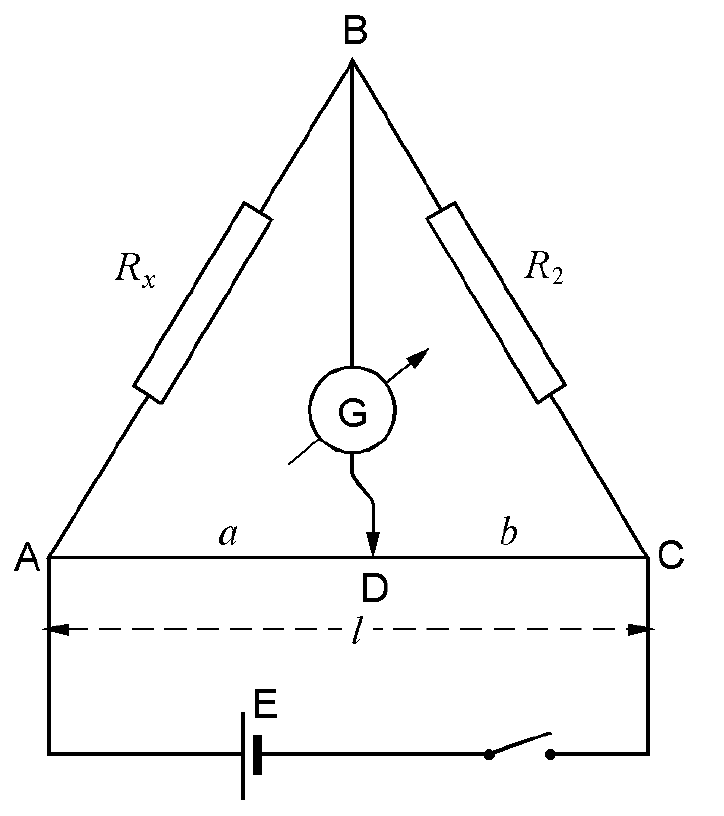
\includegraphics[scale=0.2]{schemat}
		\caption{Schemat elektryczny mostka \\ \textit{Źródło: Pracownia Fizyczna WFiIS AGH - „Ćwiczenie nr 32: Mostek Wheatstone'a”} }
		\label{schematUkladu}
	\end{figure}
	
%--------------------------------------------------------------------------------------------------------------

	\newpage
	\section{Wykonanie ćwiczenia}
	
	\begin{enumerate}
		\item Połączenie układu elektrycznego według schematu
		\item Wykonanie pomiarów wszystkich nieznanych oporników wmontowanych w płytkę z pleksiglasu oraz zapisanie wyników do tabeli
		\item Wykonanie anologicznych pomiarów dla równoległego i szeregowego połączenia oporników oraz zapisanie wyników do tabeli
	\end{enumerate}

%--------------------------------------------------------------------------------------------------------------
	
	\section{Opracowanie danych pomiarowych}
	
	%----------------------------------------------------------------------------------------------------------	
	
	\subsection{Analiza niepewności}
	
%--------------------------------------------------------------------------------------------------------------

	\section{Podsumowanie}

%--------------------------------------------------------------------------------------------------------------

\end{document}